%----------------------------------------------------------------------------------------
% DOCUMENT CONFIGURATION
%----------------------------------------------------------------------------------------
\documentclass[10pt,english,french]{article}

%----------------------------------------------------------------------------------------
% ENCODING
%----------------------------------------------------------------------------------------
\usepackage[T1]{fontenc}
\usepackage[utf8]{inputenc}
\usepackage[USenglish, french]{isodate}
\usepackage{fancyhdr}
\usepackage[numbers]{natbib}

%----------------------------------------------------------------------------------------
% LOGIC
%----------------------------------------------------------------------------------------
\usepackage{xstring, xifthen}
\usepackage{enumitem}
\usepackage[english, french]{babel}
\usepackage{blindtext}
\usepackage{pdfpages}
\usepackage{changepage}
\usepackage{etoolbox}
\usepackage{tabularx}

%----------------------------------------------------------------------------------------
% FONT SETTINGS
%----------------------------------------------------------------------------------------
% -------> Roboto
% \usepackage[sfdefault]{roboto}
% \renewcommand*\familydefault{\sfdefault}
% \renewcommand{\familydefault}{\sfdefault}
% \usepackage{moresize}
% -------> TeX Gyre Heros
% \usepackage{tgheros}
% \renewcommand{\familydefault}{\sfdefault}
% -------> Source Sans Pro
% \usepackage[default]{sourcesanspro}
% \renewcommand*\familydefault{\sfdefault}
% -------> To use LaTeX default font do not include any font package

%----------------------------------------------------------------------------------------
% ICONS / EMOJIS
%----------------------------------------------------------------------------------------
\usepackage{xparse}
\usepackage{twemojis}
\usepackage{fontawesome5}
\usepackage{xcolor}

% Icon shortcut
\newcommand{\icon}[3]{\makebox(#2,#2){\textcolor{deep_blue}{\csname fa#1\endcsname}}}
% Icon with text shortcut
\newcommand{\icontext}[4]{\vcenteredhbox{\icon{#1}{#2}{#3}}\hspace{2pt}\parbox{0.9\mpwidth}{\textcolor{#4}{#3}}}

% Define custom commands for colored icons
\newcommand{\linkedinIcon}[1][black]{\textcolor{#1}{\faLinkedin}}
\newcommand{\githubIcon}[1][black]{\textcolor{#1}{\faGithub}}
\newcommand{\emailIcon}[1][black]{\textcolor{#1}{\faEnvelope}}
\newcommand{\emailLink}[2][black]{\href{mailto:#2}{\emailIcon[black] \textcolor{#1}{#2}}}
\newcommand{\locationIcon}[1][black]{\textcolor{#1}{\faMapMarker}}
\newcommand{\phoneIcon}[1][black]{\textcolor{#1}{\faPhone}}
\newcommand{\checkIcon}[1][black]{\textcolor{#1}{\faCheck}}
\newcommand{\chessIcon}[1][black]{\textcolor{#1}{\faChess}}
\newcommand{\skiIcon}[1][black]{\textcolor{#1}{\faSkiing}}
\newcommand{\cryptoIcon}[1][black]{\textcolor{#1}{\faBitcoin}}
\newcommand{\swimmingIcon}[1][black]{\textcolor{#1}{\faSwimmer}}
\newcommand{\mountainsIcon}[1][black]{\textcolor{#1}{\faMountain}}
\newcommand{\hourglassIcon}[1][black]{\textcolor{#1}{\faHourglassHalf}}
\newcommand{\calendarCheckIcon}[1][black]{\textcolor{#1}{\faCalendarCheck}}
\newcommand{\goalIcon}[1][black]{\textcolor{#1}{\faBullseye}}
\newcommand{\educationIcon}[1][black]{\textcolor{#1}{\faGraduationCap}}
\newcommand{\birthdayIcon}[1][black]{\textcolor{#1}{\faUser}}
\newcommand{\nationalityIcon}[1][black]{\textcolor{#1}{\faGlobe}}
\newcommand{\workIcon}[1][black]{\textcolor{#1}{\faBriefcase}}
\newcommand{\itProjectIcon}[1][black]{\textcolor{#1}{\faLaptopCode}}
\newcommand{\awardIcon}[1][black]{\textcolor{#1}{\faTrophy}}
\newcommand{\circlednumber}[1][black]{\textcircled{\raisebox{-0.9pt}{#1}}}
\newcommand{\gearIcon}[1][black]{\textcolor{#1}{\faCog}}
\newcommand{\speechBubbleIcon}[1][black]{\textcolor{#1}{\faComment}}
\newcommand{\certificateIcon}[1][black]{\textcolor{#1}{\faClipboard}}
\newcommand{\starIcon}[1][black]{\textcolor{#1}{\faStar}}
\newcommand{\tradingIcon}[1][black]{\textcolor{#1}{\faChartBar}}

%----------------------------------------------------------------------------------------
% PAGE LAYOUT DEFINITIONS
%----------------------------------------------------------------------------------------
%-------------------------------------
% page outer frames for debugging
% \usepackage{showframe}
%-------------------------------------
\usepackage{paracol}
\usepackage{tikzpagenodes}
\usetikzlibrary{calc}
\usepackage{lmodern}
\usepackage{multicol}
\usepackage{lipsum}
\usepackage{atbegshi}
\usepackage[a4paper]{geometry}
\geometry{top=0.25cm, bottom=0.0625cm, left=0.1875cm, right=0.1875cm}

\pagestyle{empty}
\setlength{\parindent}{0mm}

%----------------------------------------------------------------------------------------
% TABLE / ARRAY DEFINITIONS
%----------------------------------------------------------------------------------------
\usepackage{array}
\newcolumntype{x}[1]{>{\raggedleft\hspace{0pt}}p{#1}}

%----------------------------------------------------------------------------------------
% GRAPHICS DEFINITIONS
%----------------------------------------------------------------------------------------
\usepackage{graphicx}
\usepackage{wrapfig}
\usepackage{float}
\floatstyle{boxed}
\restylefloat{figure}
\usepackage{tikz}
\usepackage{ragged2e}
\usetikzlibrary{shapes, backgrounds, mindmap, trees}

%----------------------------------------------------------------------------------------
% COLOR DEFINITIONS
%----------------------------------------------------------------------------------------
\usepackage{transparent}
\usepackage{color}
\usepackage[most]{tcolorbox}
% natural colors
\definecolor{black}{RGB}{0, 0, 0}
\definecolor{white}{RGB}{255, 255, 255}
\definecolor{blue}{RGB}{46, 134, 193}
\definecolor{brown}{RGB}{175, 96, 26}
% deep colors
\definecolor{deep_blue}{RGB}{52, 73, 94}
\definecolor{middle_deep_blue}{RGB}{46, 134, 193}
\definecolor{deep_green}{RGB}{34, 153, 84}
\definecolor{deep_grey}{RGB}{113, 125, 126}
% light colors
\definecolor{light_gray}{RGB}{245, 245, 245}
\definecolor{middle_light_gray}{RGB}{230, 230, 230}
\definecolor{light_orange}{RGB}{230, 126, 34}
\definecolor{light_green}{RGB}{234, 250, 241}
\definecolor{light_beige}{RGB}{253, 242, 233}
\definecolor{light_yellow}{RGB}{255, 255, 204}
% additional colors
\definecolor{soft_coral}{RGB}{255, 152, 133}
\definecolor{light_aqua}{RGB}{173, 232, 244}
\definecolor{teal}{RGB}{38, 170, 165}
\definecolor{middle_blue}{RGB}{84, 153, 199}

%----------------------------------------------------------------------------------------
% LINKS
%----------------------------------------------------------------------------------------
\usepackage{url}                                                
\usepackage[hidelinks]{hyperref}
% \usepackage[colorlinks=true, linkcolor=blue, citecolor=blue, urlcolor=blue, filecolor=blue]{hyperref}                                           
% \usepackage[colorlinks=false]{hyperref}
% added to ensure correct hyperlinks                                
\phantomsection{}
\usepackage{bookmark}

%-------------------------------------------------------------------------------------------------------
% AVOID WARNINGS
%-------------------------------------------------------------------------------------------------------
% chktex-file 12
% to avoid'Underfull \hbox (badness 10000)LaTeX' which reports issues with text distribution across lines or pages
\hbadness=10001

%----------------------------------------------------------------------------------------
% CV COMMANDS
%----------------------------------------------------------------------------------------
\newlength{\mpwidth}
\setlength{\mpwidth}{\textwidth}

\newcommand{\cvname}[1]{
    \begin{center}
        \textbf{\textcolor{black}{\fontsize{17pt}{12pt}\selectfont #1}}
    \end{center}
}

\newcommand{\cvsection}[1]{
    \vspace{4pt}
    \textbf{\fontsize{12pt}{10pt}\selectfont \textcolor{black}{#1}}
    \vspace{6pt}
    \hrule
    \vspace{6pt}
}

\newcommand{\cvtext}[1]{
    \begin{tabular*}{1\mpwidth}{p{0.98\mpwidth}}
        \parbox{1\mpwidth}{#1}
    \end{tabular*}
}

\newcommand{\cvtextnotab}[1]{
    \parbox{1\mpwidth}{#1}
}

% the first argument is the event; the second is the date range
\newcommand{\cvevent}[2]{
    \vspace{2pt}
    \parbox{\mpwidth}{
        \begin{tabular*}{1\mpwidth}{@{\extracolsep{\fill}} l r}
            \textcolor{black}{\textbf{\fontsize{11}{12}\selectfont #1}} & \textcolor{black}{\textbf{\fontsize{12}{12}\selectfont #2}} \\
        \end{tabular*}\\[-8pt] % to reduced some space
    }
}

% the first argument is the event; the second is the language and precision; the third is the date range
\newcommand{\cveventitproject}[3]{
    \vspace{2pt}
    \parbox{\mpwidth}{
        \begin{tabular*}{\mpwidth}{@{\extracolsep{\fill}} l r}
            \textcolor{black}{\textbf{\fontsize{11}{12}\selectfont #1}}\hspace{-5pt}\textbf{\textcolor{black}{\quad|\quad}}\hspace{-5pt}\textcolor{black}{\textit{\fontsize{11}{12}\selectfont #2}} & 
            \textcolor{black}{\textbf{\fontsize{12}{12}\selectfont #3}} \\
        \end{tabular*}\\[-8pt] % to reduce space
    }
}

% the first argument is the speciality; the second is the place
\newcommand{\cvsubevent}[2]{
    \parbox{\mpwidth}{
        \begin{tabular*}{1\mpwidth}{@{\extracolsep{\fill}} l r}
            \textcolor{black}{\textit{\fontsize{10}{12}\selectfont #1}} & \textcolor{black}{\textit{\fontsize{10}{12}\selectfont #2}} \\
        \end{tabular*}\\[-8pt] % to reduced some space
    }
    \vspace{-10pt}
}

\newcommand{\cvcourses}[2]{
    \begin{tabularx}{\mpwidth}{@{}lX@{}}
        \textcolor{black}{\textbf{\fontsize{10}{12}\selectfont #1}} & \textcolor{black}{\fontsize{10}{12}\selectfont #2}
    \end{tabularx}
    \vspace{12pt}
}

%----------------------------------------------------------------------------------------
% DOCUMENT CONTENT
%----------------------------------------------------------------------------------------
\begin{document}
\hbadness=10000     % Suppress overfull warnings globally
\sloppy             % Better line breaks
\hfuzz=10000pt      % Suppress box warnings globally

%---------------------------------------------------------------------------------------
% TITRE
%---------------------------------------------------------------------------------------
\pdfbookmark[1]{Contact}{contact}
\noindent
\begin{minipage}[c]{0.86\textwidth}
    \begin{center}
        \textbf{\textcolor{black}{\fontsize{17pt}{12pt}\selectfont Dmytro Palahin}}
    \end{center}
    \vspace{-16pt}
    \begin{center}
        {\fontsize{9pt}{11pt}\selectfont
            \locationIcon[black]\hspace{3pt}Paris, France\hspace{18pt}
            \href{tel:+33787325878}{\phoneIcon[black]\hspace{3pt}+33 7 87 32 58 78}\hspace{18pt}
            \emailLink[black]{dmytro.palahin@gmail.com}\hspace{18pt}
            \linkedinIcon[black]\hspace{3pt}\href{https://www.linkedin.com/in/dmytro-palahin/}{Dmytro Palahin}\hspace{18pt}
            \githubIcon[black]\hspace{3pt}\href{https://github.com/DmytroPalahin}{DmytroPalahin}\hspace{18pt}
            \birthdayIcon[black]\hspace{3pt}05/12/2003\hspace{18pt}
            \nationalityIcon[black]\hspace{3pt}Ukrainien
        }
    \end{center}
\end{minipage}%
\hspace{3pt}
\begin{minipage}[c]{0.11\textwidth}
    \raggedleft{}
    \begin{tikzpicture}
        \clip (0,0) circle (1.0cm);
        \node at (0,0) {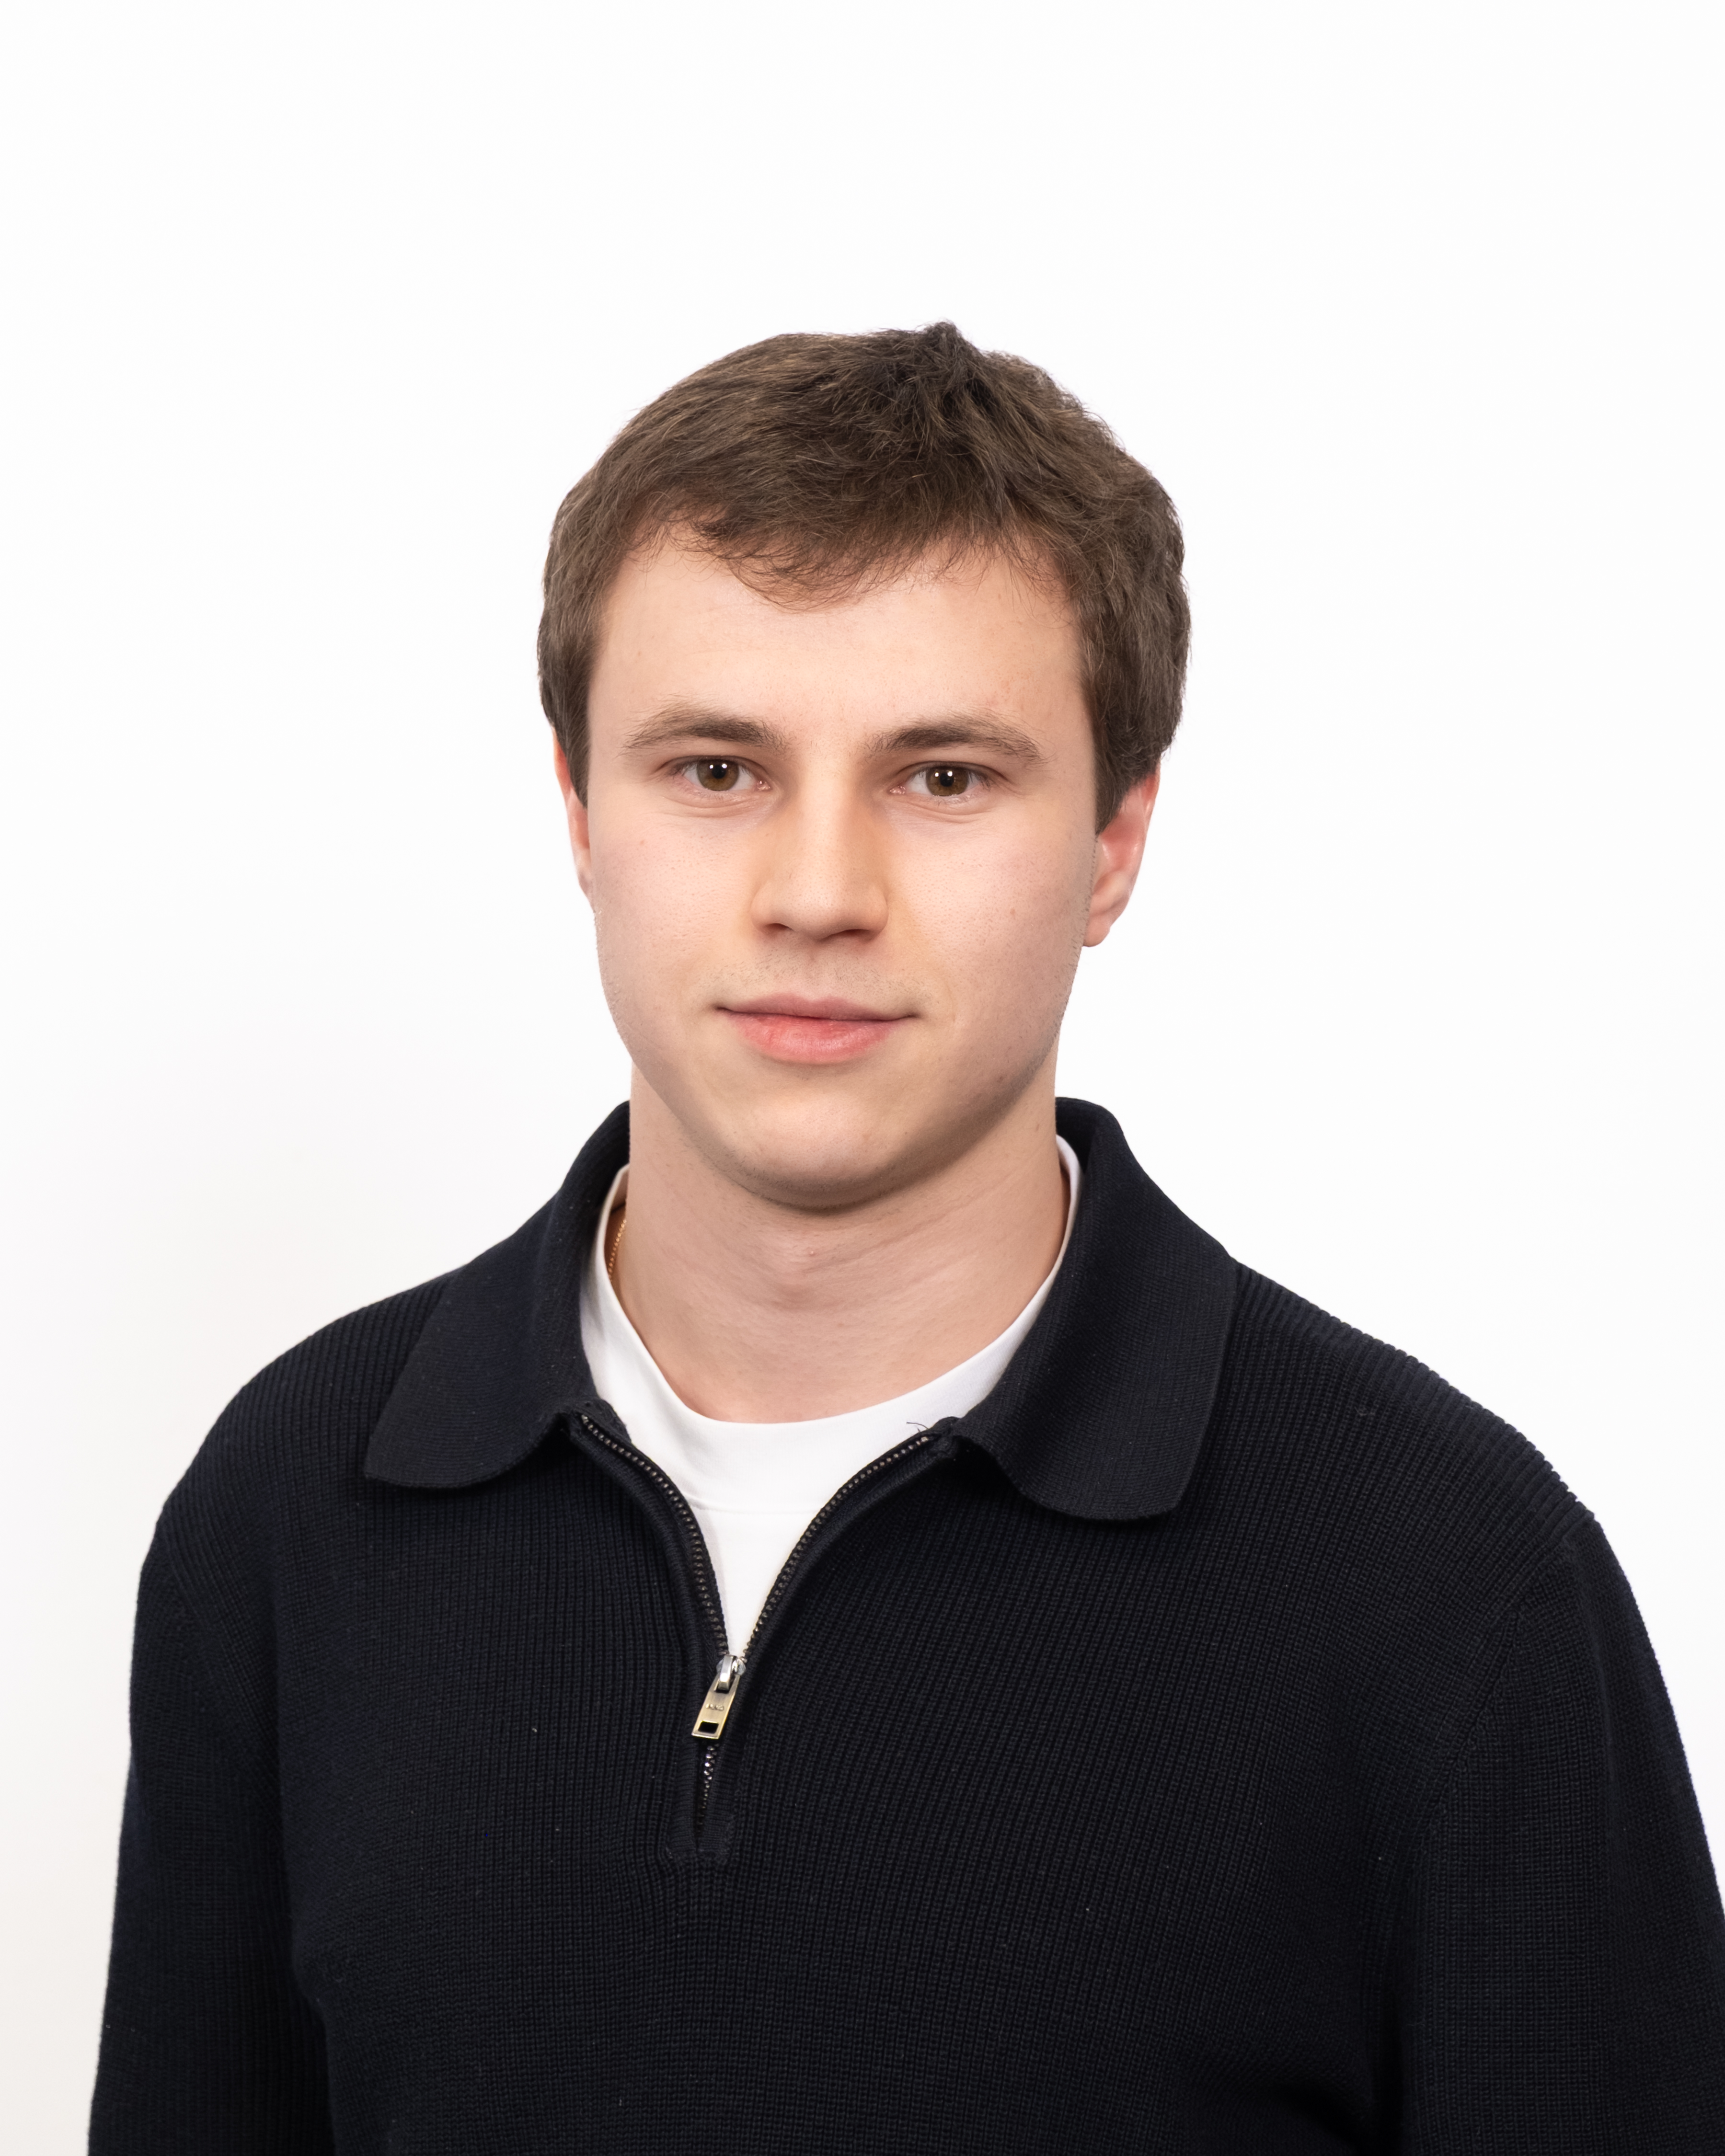
\includegraphics[width=1.6cm, keepaspectratio]{img/photo.png}};
    \end{tikzpicture}
\end{minipage}

%----------------------------------------------------------------------------------------
% FORMATION
%----------------------------------------------------------------------------------------
\vspace{-15pt}
\pdfbookmark[1]{Formation}{education}
\cvsection{\educationIcon[black]\hspace{4pt}FORMATION}

\vspace{-7pt}
\pdfbookmark[2]{Sup Galilée}{sup_galilee}
\cvevent{\href{https://www.sup-galilee.univ-paris13.fr/}{École d'ingénieurs Sup Galilée}}{2023\hspace{5pt}--\hspace{5pt}2026}
\cvsubevent{Diplôme d'ingénieur en Informatique}{Villetaneuse, France}
\cvcourses{Cours\,:}{Méthodes numériques, Structures de données, Probabilités et statistiques, Programmation orientée objet, C/C++, Python, SQL, Fouille de données, Web, Complexité, Compilation, Cloud Computing, Cybersécurité}

\vspace{-6pt}
\pdfbookmark[2]{Classe préparatoire}{prepa}
\cvevent{\href{https://www.sup-galilee.univ-paris13.fr/index.php/formation/cp2i/}{Université Sorbonne Paris Nord}}{2021\hspace{5pt}--\hspace{5pt}2023}
\cvsubevent{Classe préparatoire à \textbf{Sup Galilée}}{Villetaneuse, France}
\cvcourses{Cours\,:}{Algèbre, Analyse, Topologie et calcul différentiel, Calcul scientifique, Algorithmique, Systèmes UNIX}

\vspace{-12pt}
\pdfbookmark[2]{Lycée}{high_school}
\cvevent{Lycée Phymly}{2016\hspace{5pt}--\hspace{5pt}2021}
\cvsubevent{Spécialité Mathématiques, Physique et Informatique}{Tcherkassy, Ukraine}

%----------------------------------------------------------------------------------------
% EXPÉRIENCE PROFESSIONNELLE
%----------------------------------------------------------------------------------------
\vspace{-2pt}
\pdfbookmark[1]{Expérience}{work_exp}
\cvsection{\workIcon[black]\hspace{4pt}EXPÉRIENCE PROFESSIONNELLE}

\vspace{-4pt}
\pdfbookmark[2]{Société Générale}{sg}
\cvevent{Stage chez Société Générale Assurances}{2023\hspace{5pt}--\hspace{5pt}2026}
\cvsubevent{Data Engineer / MLOps}{La Défense, France}
\vspace{-3pt}
\begin{itemize}[leftmargin=0.5cm, label=\textbullet, itemsep=0.0625em]

    \item Développé des \textbf{extensions VSCode} (\textbf{TypeScript}) pour optimiser
          les workflows des data scientists sur la plateforme interne Data

    \item Conçu des \textbf{tableaux de bord de performance Callbot} (\textbf{Apache
              Superset}) avec des KPI personnalisés pour suivre l'efficacité et l'adoption du
          système

    \item Analysé les erreurs de reconnaissance du \textbf{Callbot Zaion}
          (\textbf{Python}) en comparant des jeux de données opérationnels ---
          identification des causes et formulation de recommandations d'amélioration

    \item Développé un \textbf{pipeline automatisé de migration de données}
          (\textbf{Python, AWS S3}) pour transférer des datasets SAS vers le cloud,
          améliorant la scalabilité et l'accès

    \item Amélioré l'outil interne de \textbf{gestion des accès} (\textbf{Python, JS})
          pour simplifier l'administration des droits des utilisateurs de la plateforme

\end{itemize}

\pdfbookmark[2]{IT Company SPD}{spd}
\vspace{-2pt}
\cvevent{Formation à l'entreprise IT SPD Ukraine}{2021}
\cvsubevent{Machine Learning / Deep Learning}{Tcherkassy, Ukraine}
\cvcourses{Outils principaux\,:}{Scikit-Learn\hspace{5pt}--\hspace{5pt}Pandas\hspace{5pt}--\hspace{5pt}Numpy\hspace{5pt}--\hspace{5pt}KNN\hspace{5pt}--\hspace{5pt}XGBoost}

%----------------------------------------------------------------------------------------
% PROJETS INFORMATIQUES
%----------------------------------------------------------------------------------------
\vspace{-10pt}
\pdfbookmark[1]{Projets}{projects}
\vspace{-1pt}
\cvsection{\itProjectIcon[black]\hspace{4pt}PROJETS INFORMATIQUES}

\vspace{-4pt}
\pdfbookmark[2]{Placement de centres logistiques}{logistics}
\cveventitproject{\href{https://github.com/DmytroPalahin/logistics-center-placement}{Placement de centres logistiques}}{Python, Julia, CPLEX, Optimisation}{2025}
{Projet d'optimisation combinatoire sur le placement de centres logistiques via des modèles MILP résolus avec CPLEX, heuristiques gloutonnes et recherche locale stochastique, avec des expériences sur des données de villes françaises et des visualisations interactives}

\vspace{1pt}
\pdfbookmark[2]{Système de réactions}{rs}
\cveventitproject{\href{https://github.com/DmytroPalahin/hsReact}{Système de réactions}}{Haskell}{2024}
{Représentation de systèmes et processus de réactions en programmation fonctionnelle}

\vspace{1pt}
\pdfbookmark[2]{Problème du voyageur}{salesman}
\cveventitproject{\href{https://github.com/DmytroPalahin/Probleme_du_Voyageur_de_Commerce}{Problème du voyageur de commerce}}{C, Apprentissage par renforcement}{2023}
{Implémentation de l'algorithme d'optimisation par colonies de fourmis}

\vspace{1pt}
\pdfbookmark[2]{Article}{article}
\cveventitproject{\href{https://www.researchsquare.com/article/rs-2203260/v1}{Publication d'un article}}{Algorithmes mathématiques}{2021}
{Méthode de filtration du bruit impulsionnel dans les images vidéo (D.Palahin, V.Palahin, O.Zorin, O.Hozhyi)\newline\textit{Informatics and Mathematical Methods in Simulation}, Vol. 11 (2021), No. 4}

\vspace{1pt}
\pdfbookmark[2]{Détection d'anomalies}{anomaly_detection}
\cveventitproject{\href{https://github.com/DmytroPalahin/Anomaly_Detection}{Détection d'anomalies}}{Python, Machine Learning}{2020}
{Méthodes pour l'étiquetage partiel de données}

\vspace{1pt}
\pdfbookmark[2]{Filtrage d'images}{filtering_imgs}
\cveventitproject{\href{https://github.com/DmytroPalahin/Filtering_Images}{Filtrage d'images}}{HTML, CSS, JS, Algorithmes}{2019}
{Implémentation de méthodes mathématiques de filtrage du bruit dans les images numériques sous forme de service web}

%----------------------------------------------------------------------------------------
% CERTIFICATIONS / COMPÉTENCES
%----------------------------------------------------------------------------------------
\vspace{3pt}
\columnratio{0.45}
\setlength{\columnsep}{1.2em}
\setlength{\columnseprule}{0pt}

\begin{paracol}{2}
    \begin{leftcolumn}
        \pdfbookmark[1]{Certifications}{certifications}
        \vspace{-1pt}
        \cvsection{\certificateIcon[black]\hspace{4pt}CERTIFICATIONS}
        \vspace{-8pt}
        \begin{itemize}[leftmargin=0.25cm, label=\textbullet, itemsep=0.0625em]
            \item \textbf{Huawei\,:} \href{https://github.com/DmytroPalahin/cv-latex-simple-en/blob/main/docs/huawei_artificial_intelligence_and_applications.pdf}{Intelligence artificielle et applications}
            \item \textbf{Huawei\,:} \href{https://github.com/DmytroPalahin/cv-latex-simple-en/blob/main/docs/huawei_artificial_intelligence_technology_and_applications.pdf}{Technologies et applications de l'IA}
            \item \textbf{SPD Ukraine\,:} Formation en Machine Learning en entreprise IT
            \item \textbf{Stepik\,:} Formation en Machine Learning
        \end{itemize}
    \end{leftcolumn}
    \begin{rightcolumn}
        \pdfbookmark[1]{Compétences}{skills}
        \vspace{-1pt}
        \cvsection{\gearIcon[black]\hspace{4pt}COMPÉTENCES}
        \vspace{-8pt}
        \begin{itemize}[leftmargin=0.25cm, label=\textbullet, itemsep=0.0625em]
            \item \textbf{ML / DL\,:} Scikit-learn, TensorFlow, Keras, XGBoost, LightGBM, CatBoost
            \item \textbf{Analyse de données\,:} Pandas, Numpy, Matplotlib, Seaborn, Plotly, Tableau, Power BI
            \item \textbf{Langages\,:} Python, C/C++, Java, SQL, HTML, JS/TS, Matlab, Haskell, Julia, LaTeX
            \item \textbf{Outils\,:} VSCode, Jupyter, Anaconda, Git, Docker, Linux, Windows, MacOS
        \end{itemize}
    \end{rightcolumn}
\end{paracol}

%----------------------------------------------------------------------------------------
% PRIX & PARTICIPATIONS / LANGUES + CENTRES D'INTÉRÊT
%----------------------------------------------------------------------------------------
\vspace{-10pt}
\columnratio{0.65}
\setlength{\columnsep}{1.2em}
\setlength{\columnseprule}{0pt}

\begin{paracol}{2}
    \pdfbookmark[1]{Participations}{participations}
    \begin{leftcolumn}
        \cvsection{\awardIcon[black]\hspace{4pt}PRIX \& PARTICIPATIONS}

        \pdfbookmark[2]{Fondation Georges Besse}{fund}
        \cvevent{Lauréat de la \href{https://www.fondationbesse.com/}{Fondation Georges Besse}}{}

        \vspace{-5pt}
        \pdfbookmark[2]{ISEF 2020}{isef}
        \cvevent{Eco\hspace{2pt}--\hspace{2pt}Techno Ukraine ISEF}{}
        {1\textsuperscript{ère} place en \textbf{Informatique} à la compétition internationale}

        \vspace{1pt}
        \pdfbookmark[2]{Collective Intelligence}{it_compt}
        \cvevent{Service Internet Intelligence Collective \textnormal{--- 1\textsuperscript{ère} place en Ukraine}}{}
    \end{leftcolumn}
    \begin{rightcolumn}
        \pdfbookmark[1]{Langues}{languages}
        \cvsection{\speechBubbleIcon[black]\hspace{4pt}LANGUES}
        \begin{tabular}{ l @{\hspace{5pt}} l @{\hspace{5pt}} l @{\hspace{5pt}} l }
            \textbf{Ukrainien} & Natif   & \textbf{Russe}   & Bilingue \\
            \textbf{Français}  & Courant & \textbf{Anglais} & Courant  \\
        \end{tabular}

        \vspace{2pt}
        \pdfbookmark[1]{Centres d'intérêt}{interests}
        \cvsection{\starIcon[black]\hspace{4pt}CENTRES D'INTÉRÊT}
        \tradingIcon[black]\hspace{2pt}Invest\hspace{6pt}
        \cryptoIcon[black]\hspace{2pt}Crypto\hspace{6pt}
        \chessIcon[black]\hspace{2pt}Échecs\hspace{6pt}
        \skiIcon[black]\hspace{2pt}Ski\hspace{6pt}
    \end{rightcolumn}
\end{paracol}

\end{document}

/*
latexmk -pdf cv-dmytro-palahin-fr.tex
latexmk -pdf -auxdir=/tmp/latex-build -outdir=. cv-dmytro-palahin-fr.tex
*/
